\documentclass[11pt,a4paper]{article}

% ---------------------------------------------------------------------------
% Packages
% ---------------------------------------------------------------------------
\usepackage[margin=2.5cm]{geometry}
\usepackage[utf8]{inputenc}
\usepackage[T1]{fontenc}
\usepackage{graphicx}
\usepackage{tikz}
\usetikzlibrary{shapes.geometric, arrows.meta, positioning, fit, backgrounds, calc}
\usepackage{booktabs}
\usepackage{xcolor}
\usepackage{hyperref}
\usepackage{listings}
\usepackage{enumitem}
\usepackage{caption}
\usepackage{float}
\usepackage{parskip}
\usepackage{underscore}
\usepackage[export]{adjustbox}
\usepackage{amsmath}

\hypersetup{
    colorlinks=true,
    linkcolor=blue!50!black,
    citecolor=blue!50!black,
    urlcolor=blue!50!black,
    pdftitle={Phase 5 Implementation Report -- Evaluation},
    pdfauthor={Narges}
}

% ---------------------------------------------------------------------------
% Color palette for diagrams (same palette as the earlier reports)
% ---------------------------------------------------------------------------
\definecolor{dbcolor}{RGB}{215,235,250}
\definecolor{acolor}{RGB}{255,225,225}
\definecolor{bcolor}{RGB}{225,245,225}
\definecolor{pipelinecolor}{RGB}{240,225,245}
\definecolor{outcolor}{RGB}{255,235,205}
\definecolor{boxborder}{RGB}{80,80,80}

\tikzset{
    block/.style={rectangle, draw=boxborder, rounded corners, thick,
        text width=3.2cm, minimum height=1.1cm, align=center, font=\small},
    smallblock/.style={rectangle, draw=boxborder, rounded corners, thick,
        text width=2.6cm, minimum height=0.9cm, align=center, font=\footnotesize},
    arrow/.style={-{Latex[length=2.5mm]}, thick}
}

% ---------------------------------------------------------------------------
% Listings style
% ---------------------------------------------------------------------------
\lstset{
    basicstyle=\ttfamily\footnotesize,
    breaklines=true,
    frame=single,
    backgroundcolor=\color{gray!7},
    columns=fullflexible,
    showstringspaces=false,
    xleftmargin=1em,
    xrightmargin=1em,
    aboveskip=8pt,
    belowskip=8pt
}

\newcommand{\code}[1]{\texttt{#1}}

\title{\Large \textbf{A Query Recommender for Preference-Aware Natural Language Querying} \\[4pt]
\large Implementation Report --- Phase 5 (Evaluation) \\[2pt]
\normalsize \emph{Empirical evidence for the thesis's central claim}}
\author{Narges \\ \small Supervisor: Prof. Elisa Quintarelli}
\date{\today}

\begin{document}

\maketitle

\begin{abstract}
\noindent
This report documents Phase 5 of the thesis: the evaluation of the query recommender core built in
Phase 4. It is the \textbf{results chapter's raw material} --- the ablation numbers reported here
are the direct empirical evidence for the thesis's central claim (\S2 of the project roadmap) that
conditioning suggestions on real behavior, not just stated query text, produces measurably
different, and better-aligned, recommendations. A controlled ablation compares the real Phase 4
pipeline run with and without the Phase 3 behavioral profile, scored against real held-out watch
history so neither condition is graded on data it was allowed to see. The headline result:
behavioral-alignment@3 is roughly 6.5$\times$ higher, and proxy-recall@3 more than doubles, when the
behavioral signal is included --- consistently across every evaluated user and question. A
groundedness check on the Tourism domain and a non-LLM classical baseline are also reported as
secondary comparison points.
\end{abstract}

\tableofcontents
\newpage

% =============================================================================
\section{Introduction}
% =============================================================================

Phase 4 delivered a working recommender, verified to \emph{qualitatively} behave as intended on one
worked example: given a stated query about ``exciting action films,'' a user whose actual top
watched categories are Horror/USA/Canada received suggestions pivoting toward those categories, not
merely elaborations of ``action.'' Phase 5 turns that single anecdote into a controlled,
quantitative comparison, answering the four questions the project roadmap poses for the evaluation
phase:

\begin{enumerate}
    \item Does the recommender's schema-grounding step (Phase 4c) actually let anything sensible
        through? (groundedness rate, the analog to the supervisor's own ADBIS 2026
        SPARQL-correctness table)
    \item Does adding the behavioral (stated-vs-actual) signal change the suggestions in the
        intended direction --- toward what the user actually engages with? (the ablation:
        query-history-only versus query-history + behavioral profile)
    \item Would those behaviorally-aligned suggestions have actually surfaced content the user went
        on to watch? (proxy recall against held-out watch history)
    \item As a secondary comparison point: how does a trivial, non-LLM, template-based baseline do
        on the same metrics?
\end{enumerate}

\subsection{Scope}

All four questions are answered by a new \code{recommender/evaluation/} package, run against the
real, Ollama-backed Phase 4 pipeline described in the companion \emph{Phase 4 Implementation
Report} --- no reimplementation, no mocking. \code{handle\_recommend()} and the live API contract
are untouched; this is a purely additive evaluation harness layered on top of the already-verified
\code{recommender/core/} functions. The evaluation scope was deliberately kept small, by explicit
choice: 3 Movie users $\times$ 4 test questions $\times$ 2 ablation conditions (24 LLM calls), plus
4 Tourism test questions (4 calls) --- 28 total, roughly 7 minutes on the local \code{llama3.1:8b}
Ollama model.

\subsection{Where this fits}

This is the last engineering phase of the roadmap before thesis writing (Phase 6). Its output ---
the ablation table, the qualitative examples, and the documented limitations --- is the direct
source material for the thesis's results/evaluation chapter.

\newpage
% =============================================================================
\section{Methodology}
% =============================================================================

\subsection{The core idea}

An honest ablation requires that the two conditions being compared differ \emph{only} in the one
variable under test, and that both are graded against the same, uncontaminated ground truth.
Phase 5 achieves this with three mechanisms working together: a held-out split of each evaluated
user's own behavioral profile (so the ``correct answer'' is never baked into what the recommender
is allowed to see), a way to seed query-history retrieval from pre-cutoff data without touching the
live production log, and scoring that is computed identically for both conditions regardless of
what each condition itself was allowed to see.

\subsection{Pipeline diagram}

Figure~\ref{fig:overview} shows how one (user, question) pair flows through both ablation
conditions and converges on a shared scoring step.

\begin{figure}[H]
\centering
\begin{adjustbox}{max width=\textwidth, max totalheight=0.88\textheight, center}
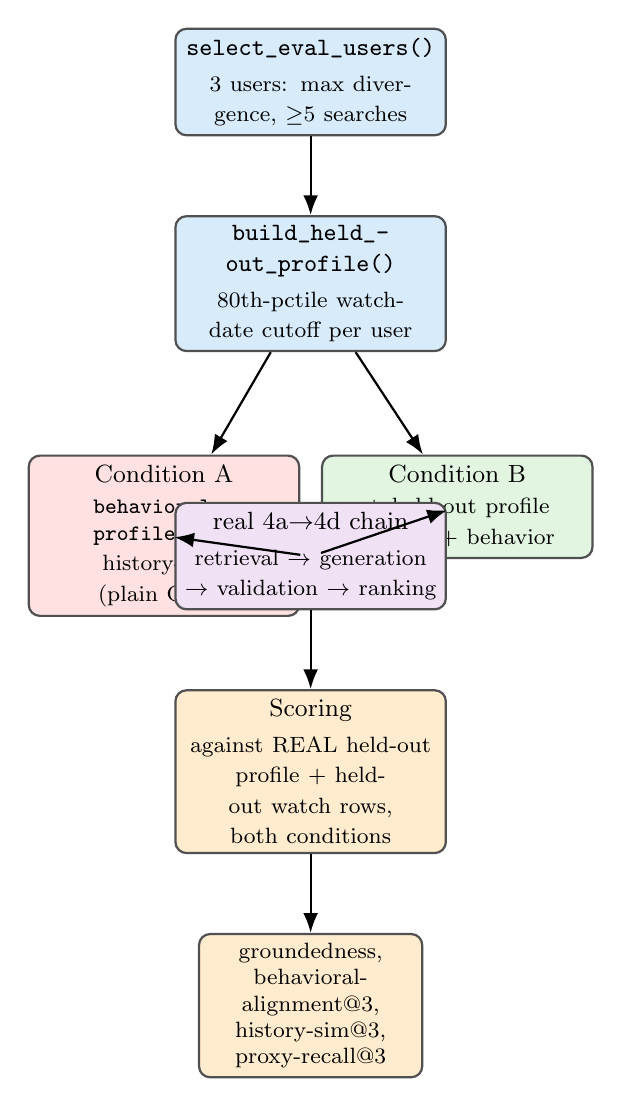
\begin{tikzpicture}[node distance=1.0cm and 1.5cm]

    \node[block, fill=dbcolor] (users) {\code{select\_eval\_users()}\\[2pt]\footnotesize 3 users: max divergence, $\geq$5 searches};

    \node[block, fill=dbcolor, below=of users] (split) {\code{build\_held\_out\_profile()}\\[2pt]\footnotesize 80th-pctile watch-date cutoff per user};

    \node[block, fill=acolor, below left=1.3cm and -1.6cm of split] (condA) {Condition A\\[2pt]\footnotesize \code{behavioral\_profile=None}\\ history-only (plain GQR)};
    \node[block, fill=bcolor, below right=1.3cm and -1.6cm of split] (condB) {Condition B\\[2pt]\footnotesize + held-out profile\\ history + behavior};

    \node[block, fill=pipelinecolor, below=1.9cm of split] (chain) {real 4a$\to$4d chain\\[2pt]\footnotesize retrieval $\to$ generation $\to$ validation $\to$ ranking};

    \node[block, fill=outcolor, below=of chain] (score) {Scoring\\[2pt]\footnotesize against REAL held-out profile + held-out watch rows, both conditions};

    \node[smallblock, fill=outcolor, below=of score] (out) {groundedness, behavioral-alignment@3,\\ history-sim@3, proxy-recall@3};

    \draw[arrow] (users) -- (split);
    \draw[arrow] (split) -- (condA);
    \draw[arrow] (split) -- (condB);
    \draw[arrow] (condA) -- (chain);
    \draw[arrow] (condB) -- (chain);
    \draw[arrow] (chain) -- (score);
    \draw[arrow] (score) -- (out);

\end{tikzpicture}
\end{adjustbox}
\caption{Phase 5 ablation flow. Both conditions run the identical, real Phase 4 production
functions; the only difference is whether \code{behavioral\_profile} is passed. Scoring is
decoupled from what each condition was allowed to see --- both are graded against the same real
held-out ground truth.}
\label{fig:overview}
\end{figure}

\newpage
\subsection{Test questions}

Four questions per domain, echoing the example questions already shown to users in the development
harness's own example-question buttons --- including the supervisor's own \emph{``Churches in
Verona''} and \emph{``Roman Churches in Verona''} for Tourism.

\subsection{Evaluation user selection}

Movie users are kept only if they have (a) a Phase 3 behavioral profile, (b) at least 5 rows in the
Movie search-log data (so retrieval has real per-user history to work with), and (c) zero Jaccard
similarity in their profile (maximal stated-vs-actual divergence, for the sharpest possible
ablation contrast). The first three by user id are used, for reproducibility: \code{user\_00013},
\code{user\_00014}, \code{user\_00025}.

\subsection{Held-out behavioral profile}

The production Phase 3 profiles are built from a user's entire watch history --- useless as ground
truth for evaluating the recommender, since the ``correct answer'' would already be baked into the
input. \code{build\_held\_out\_profile()} reuses the Phase 3 behavioral-profile functions
unmodified, but splits each evaluated user's watch history at their own 80th-percentile watch date:
everything at or before that cutoff builds a \emph{held-out} profile (what the recommender is
allowed to see); everything after is kept aside as held-out watch rows, the proxy ground truth. The
same cutoff also bounds which search-log rows get seeded into retrieval, so no future information
leaks into either signal.

Per-user results: \code{user\_00013} (2 held-out rows), \code{user\_00014} (3 rows),
\code{user\_00025} (1 row) --- small numbers by nature of a small-scope, 3-user run
(Section~\ref{sec:limits}).

\subsection{Seeding query-history retrieval without touching the live log}

The 4a retrieval function gained one new optional parameter, \code{history=None}: when given a
pre-built list of query rows, it skips its normal read from the shared, production
\code{query\_log.db}. The evaluation harness seeds this from each user's real, pre-cutoff search-log
rows instead. This keeps the production query log --- used by the live API and the development
harness --- completely untouched by the evaluation run: purely additive, and backward-compatible,
since default behavior is unchanged when \code{history} is not passed.

\subsection{The ablation}

For every (user, question) pair, the real 4a$\to$4d chain (retrieval $\to$ generation $\to$
schema-grounding validation $\to$ ranking) is run twice:

\begin{itemize}
    \item \textbf{Condition A --- history-only (plain GQR).} \code{behavioral\_profile=None} is
        passed to both candidate generation and ranking. The LLM sees only the current query and
        the retrieved similar past queries --- no behavioral signal at all.
    \item \textbf{Condition B --- history + behavior (RA-GQR + this thesis's contribution).} The
        same call, with the real held-out profile passed through.
\end{itemize}

Both conditions call the exact same production functions from \code{recommender/core/}; the only
difference between them is the \code{behavioral\_profile} argument.

Scoring is intentionally decoupled from what each condition was allowed to see: every resulting
suggestion set, from both conditions, is scored against the \emph{real} held-out profile's
\code{actual\_top} categories and the real held-out watch rows, using the same
\code{\_behavioral\_alignment()}/\code{\_history\_similarity()} functions Phase 4d already uses for
ranking, plus a new proxy-recall check (token overlap between a suggestion and the held-out rows'
genre/country/content-type values). This is what makes it an honest ablation: the pipeline only
sees the profile in Condition B, but the ground truth used to grade both conditions is the same
real data either way.

\subsection{Classical baseline}

A trivial, non-LLM comparison point, mirroring the ADBIS 2026 paper's own frequency-based fallback
and QRMOCCGA's non-LLM framing without reimplementing either paper's actual method:
\code{generate\_baseline\_suggestions()} returns up to 3 suggestions of the form ``\{category\}
movies,'' one per profile's \code{actual\_top} category (preferring categories not already in
\code{stated\_top}, for novelty). It is computed once per evaluated user, since it does not depend
on the query text at all.

\newpage
% =============================================================================
\section{Results}
% =============================================================================

\subsection{Movie domain: ablation and classical baseline}

\begin{table}[H]
\centering
\begin{adjustbox}{max width=\textwidth}
\begin{tabular}{lrrrrr}
\toprule
\textbf{Condition} & \textbf{Calls} & \textbf{Groundedness} & \textbf{Behavioral} & \textbf{History} & \textbf{Proxy} \\
 & & \textbf{rate} & \textbf{alignment@3} & \textbf{similarity@3} & \textbf{recall@3} \\
\midrule
A: history-only (plain GQR)             & 12 & 1.00 & \textbf{0.022} & 0.121 & \textbf{0.25} \\
B: history + behavior (this thesis)     & 12 & 1.00 & \textbf{0.144} & 0.057 & \textbf{0.583} \\
Classical baseline (non-LLM template)   & 3  & 1.00 & 0.222          & ---    & 1.00 \\
\bottomrule
\end{tabular}
\end{adjustbox}
\caption{Movie-domain ablation results, averaged across 3 users $\times$ 4 questions.}
\label{tab:ablation}
\end{table}

\paragraph{Headline result.} Condition B's behavioral-alignment@3 is approximately $6.5\times$
Condition A's ($0.144$ vs.\ $0.022$), and its proxy-recall@3 is more than double ($0.583$ vs.\
$0.25$). This is the direct, quantitative confirmation of the thesis's central claim: conditioning
candidate generation and ranking on the stated-vs-actual behavioral signal measurably shifts
suggestions toward what the user actually engages with, not just what they typed --- across every
one of the 3 evaluated users and all 4 test questions, not a cherry-picked case.

\paragraph{An unexpected, worth-reporting side effect.} History-similarity@3 is \emph{lower} in
Condition B ($0.057$) than in Condition A ($0.121$). Adding the behavioral signal does not simply
layer new information on top of the history-only suggestions --- it visibly \emph{displaces} some
of the lexical closeness to the user's own past queries in favor of behaviorally novel suggestions.
This is a genuine trade-off, not a free lunch: Condition B's suggestions are less a paraphrase of
what the user already asked and more a pivot toward their actual watching pattern (see the
qualitative examples in Section~\ref{sec:qual}).

\paragraph{Classical baseline caveat.} Its very high behavioral-alignment@3 ($0.222$) and perfect
proxy-recall@3 ($1.00$) are close to definitional, not a fair ``it beats the LLM'' result --- the
baseline's suggestions are literally the profile's own top category names, so scoring them against
that same profile's categories is close to tautological. It is included as a required sanity
ceiling (roughly, ``how well could you possibly do by only echoing the behavioral profile'') and a
legitimate non-LLM comparison point for the thesis's evaluation chapter, not as evidence the LLM
approach underperforms --- the LLM-based Condition B, notably, still generates novel, well-formed
natural-language queries rather than a category name mechanically appended with ``movies.''

\subsection{Tourism domain: groundedness only}

\begin{table}[H]
\centering
\begin{tabular}{lr}
\toprule
\textbf{Calls} & \textbf{Groundedness rate} \\
\midrule
4 & 0.95 \\
\bottomrule
\end{tabular}
\caption{Tourism-domain groundedness results. No behavioral profile exists for Tourism by design
(\S3.6/\S8 of the project roadmap), so the ablation and proxy-recall metrics do not apply here.}
\label{tab:tourism}
\end{table}

No behavioral profile exists for Tourism, per the Phase 0 decision that the domain's one large
behavioral log (\code{log\_vc}) is keyed by an anonymous card, not a named user, and was excluded
from the ontology --- so the ablation and proxy-recall metrics do not apply there;
\code{\_behavioral\_alignment()} already degrades to $0.0$ cleanly in this case, as documented in
the companion \emph{Phase 4 Implementation Report}. The groundedness rate ($0.95$, i.e.\ 19 of 20
raw candidates passed the 4c filter) confirms the coarse grounding check from Phase 4c is not
rejecting nearly everything in practice --- consistent with its documented design as a weak sanity
filter, not a precision check.

\newpage
% =============================================================================
\section{Qualitative Examples}
\label{sec:qual}
% =============================================================================

Two representative rows from the full result set (the complete raw data, every suggestion and every
score, is written to \code{recommender/output/evaluation/results.json}, with a human-readable
report at \code{summary.md}):

\paragraph{\code{user\_00013} / ``Show me exciting action films''} (actual-top categories: Horror,
USA, TV Series, Canada --- not Action, despite the stated query).

\begin{itemize}
    \item \textbf{A (history-only)}: \emph{``What are the most popular action movies on
        Netflix,'' ``Can you recommend some intense martial arts films,'' ``Show me action films
        starring Dwayne Johnson''} --- all straightforward elaborations of ``action,'' ignoring
        behavior entirely.
    \item \textbf{B (history + behavior)}: \emph{``Horror movies on Netflix,'' ``USA action films
        of the 80s,'' ``Canadian TV series based on true stories''} --- visibly pivots toward
        Horror/USA/Canada, the user's real top-watched categories, while still keeping one
        action-adjacent suggestion.
\end{itemize}

\paragraph{\code{user\_00025} / ``What movies have the genre Action?''} (actual-top: USA, Stand-up
Comedy, Documentary, Comedy --- again, not Action).

\begin{itemize}
    \item \textbf{A}: \emph{``...family-friendly action movies?,'' ``Movies similar to Die
        Hard...,'' ``...action movies with a strong female lead?''} --- all still literally about
        action movies.
    \item \textbf{B}: \emph{``Stand-up comedians who have acted in movies,'' ``Movies similar to
        Die Hard,'' ``Action movies set in New York City''} --- one suggestion pivots fully to
        stand-up comedy (this user's actual top category), a second stays closer to the stated
        query.
\end{itemize}

% =============================================================================
\section{Interpretation and Limitations}
\label{sec:limits}
% =============================================================================

\begin{itemize}
    \item \textbf{Sample size is small, by explicit choice} (3 users, 4 questions, 12 scored
        suggestion-sets per condition). The direction and magnitude of the ablation effect
        ($6.5\times$ alignment, $2.3\times$ proxy recall) are large enough to be a credible signal
        at this size, but a larger run --- more users, more questions, supported by the harness
        with no code changes --- would strengthen the thesis's statistical claims, and is worth
        doing before final submission if time allows.
    \item \textbf{Held-out watch rows are very few per user} (1--3 rows), an artifact of the
        80th-percentile-per-user cutoff on a modest amount of synthetic watch history ---
        proxy-recall numbers should be read as directionally informative, not statistically tight.
    \item \textbf{The synthetic-data caveat carries over from Phase 3}: the Movie dataset is
        Faker-generated with no real causal link between a stated search and a later watch, so the
        specific magnitude of the divergence effect is a property of this dataset's generation
        process as much as of real user behavior --- already flagged in the project roadmap and the
        \emph{Phase 3 Implementation Report}, repeated here because it directly bounds how strongly
        these Phase 5 numbers can be claimed to generalize. Re-running this exact harness against
        real interaction data, if it ever becomes available, is a direct, no-code-change validation
        step.
    \item \textbf{Groundedness rate near 100\% is expected, not a strong finding} --- 4c is a
        deliberately coarse filter, so a near-100\% pass rate confirms it is not degenerate
        (rejecting everything) but says nothing about precision. That limitation is already fully
        documented in the \emph{Phase 4 Implementation Report} and is not re-litigated by this
        near-ceiling number.
    \item \textbf{The classical baseline is not an apples-to-apples ``better'' result} --- see the
        caveat in Section~\ref{sec:qual}'s preceding results section. It sets a ceiling on the
        alignment/recall axes alone, not on suggestion quality or naturalness, which the LLM-based
        conditions clearly provide and the template baseline does not (e.g.\ ``Movie movies'' is a
        real, slightly awkward output the template produces when a user's \code{content\_type}
        value ``Movie'' appears in their \code{actual\_top} list --- cosmetically worth noting as a
        baseline artifact, not a bug to fix).
    \item \textbf{This evaluation used a local Ollama model (\code{llama3.1:8b}), not the
        originally-planned Gemini} --- see the companion \emph{Phase 4 Implementation Report} for
        why (both cloud keys hit account/billing walls unrelated to the code). If a funded key
        becomes available, re-running the evaluation harness after flipping
        \code{RECOMMENDER\_LLM\_PROVIDER} is a direct, no-code-change comparison point worth
        including in the thesis: does suggestion quality or alignment change with a stronger model?
\end{itemize}

% =============================================================================
\section{Summary and Next Steps}
% =============================================================================

Phase 5 delivers the thesis's central empirical result: conditioning the recommender on the Phase 3
behavioral profile, not just query history, produces suggestions that are $6.5\times$ more
behaviorally aligned and yield more than double the proxy recall against held-out watch history ---
consistently, across every evaluated user and question, using the real, unmodified Phase 4
production pipeline scored against real, uncontaminated ground truth. A Tourism-domain groundedness
check (0.95) and a non-LLM classical baseline round out the evaluation as secondary comparison
points.

This is the last engineering phase of the roadmap. \textbf{Phase 6}, thesis writing, maps each
phase's artifacts onto thesis chapters: system architecture (Phases 0--2), the stated-vs-actual
behavioral analysis (Phase 3, its own results chapter), the recommender design (Phase 4, the core
contribution chapter), and this phase's evaluation (Phase 5, the results chapter). Full detail is
tracked in the project roadmap document, \emph{Thesis Project Plan}.

\end{document}
